\documentclass{standalone}

\usepackage{tikz}
\usepackage{circuitikz}

\tikzset{block/.style = {draw, fill=white, very thick, rectangle, minimum height=1cm, minimum width=2cm},
         lblock/.style={draw,fill=white,very thick, rectangle, minimum height=3cm, minimum width=1cm},
         sum/.style= {draw, fill=white, very thick, circle, node distance=0.5cm}}

         
\begin{document}
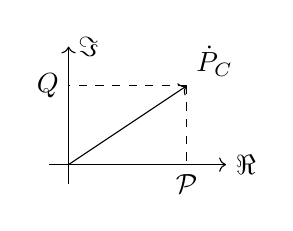
\begin{tikzpicture}
    \draw[->](-0.25,0)--(2,0)node[right]{$\Re$};
    \draw[->](0,-0.25)--(0,1.5)node[right]{$\Im$};

    \draw[->](0,0)--(1.5,1)node[above right]{$\dot P_C$};
    \draw[dashed](1.5,1)--(0,1)node[left]{$Q$};
    \draw[dashed](1.5,1)--(1.5,0)node[below]{$\mathcal{P}$};
\end{tikzpicture}
\end{document}